\documentclass[aspectratio=169]{beamer}
\usefonttheme[onlymath]{serif}
\mode<presentation> {
\usetheme[hideallsubsections]{Berkeley}
\usecolortheme{orchid}

%\setbeamertemplate{footline} % To remove the footer line in all slides uncomment this line
\setbeamertemplate{footline}[page number] % To replace the footer line in all slides with a simple slide count uncomment this line
\setbeamertemplate{navigation symbols}{} % To remove the navigation symbols from the bottom of all slides uncomment this line
}

\usepackage[export]{adjustbox}
\usepackage{amssymb}
\usepackage{bigints}
\usepackage{booktabs}
\usepackage{graphicx}
\usepackage{hyperref}
\usepackage{mathtools}
\usepackage[percent]{overpic}
\usepackage{relsize}
\usepackage{subcaption}

% manage toc animations
\usepackage{totcount}
\regtotcounter{section}
\usepackage{multido}

%\newcommand{\mytableofcontents}[0]{
%\multido{\I=1+1}{\totvalue{section}}{
%  \begin{frame}<beamer>
%  \setcounter{section}{\I}
%  \frametitle{Outline}
%  \tableofcontents[
%    currentsection,
%    sectionstyle=show/show,
%    subsectionstyle=show/show/hide,
%  ]
%  \end{frame}
%}
%\setcounter{section}{0}
%}

%----------------------------------------------------------------------------------------
%	TITLE PAGE
%----------------------------------------------------------------------------------------

\title[GATs]{Graph Attention Networks} % The short title appears at the bottom of every slide, the full title is only on the title page

\author{Justin Pauckert}
\institute[TUB]
{Discrete Optimization and Machine Learning \\
TU Berlin \\
}

\begin{document}

\begin{frame}
    \titlepage
\end{frame}

%\mytableofcontents
%----------------------------------------------------------------------------------------
%	PRESENTATION SLIDES
%----------------------------------------------------------------------------------------

%------------------------------------------------
\section[NN for Graphs]{Neural Networks for Graphs}
%------------------------------------------------
\subsection{Problem Setup}
\begin{frame}
    \frametitle{Graph Data}
    \begin{columns}
        \column{.5\textwidth}
            \centering
            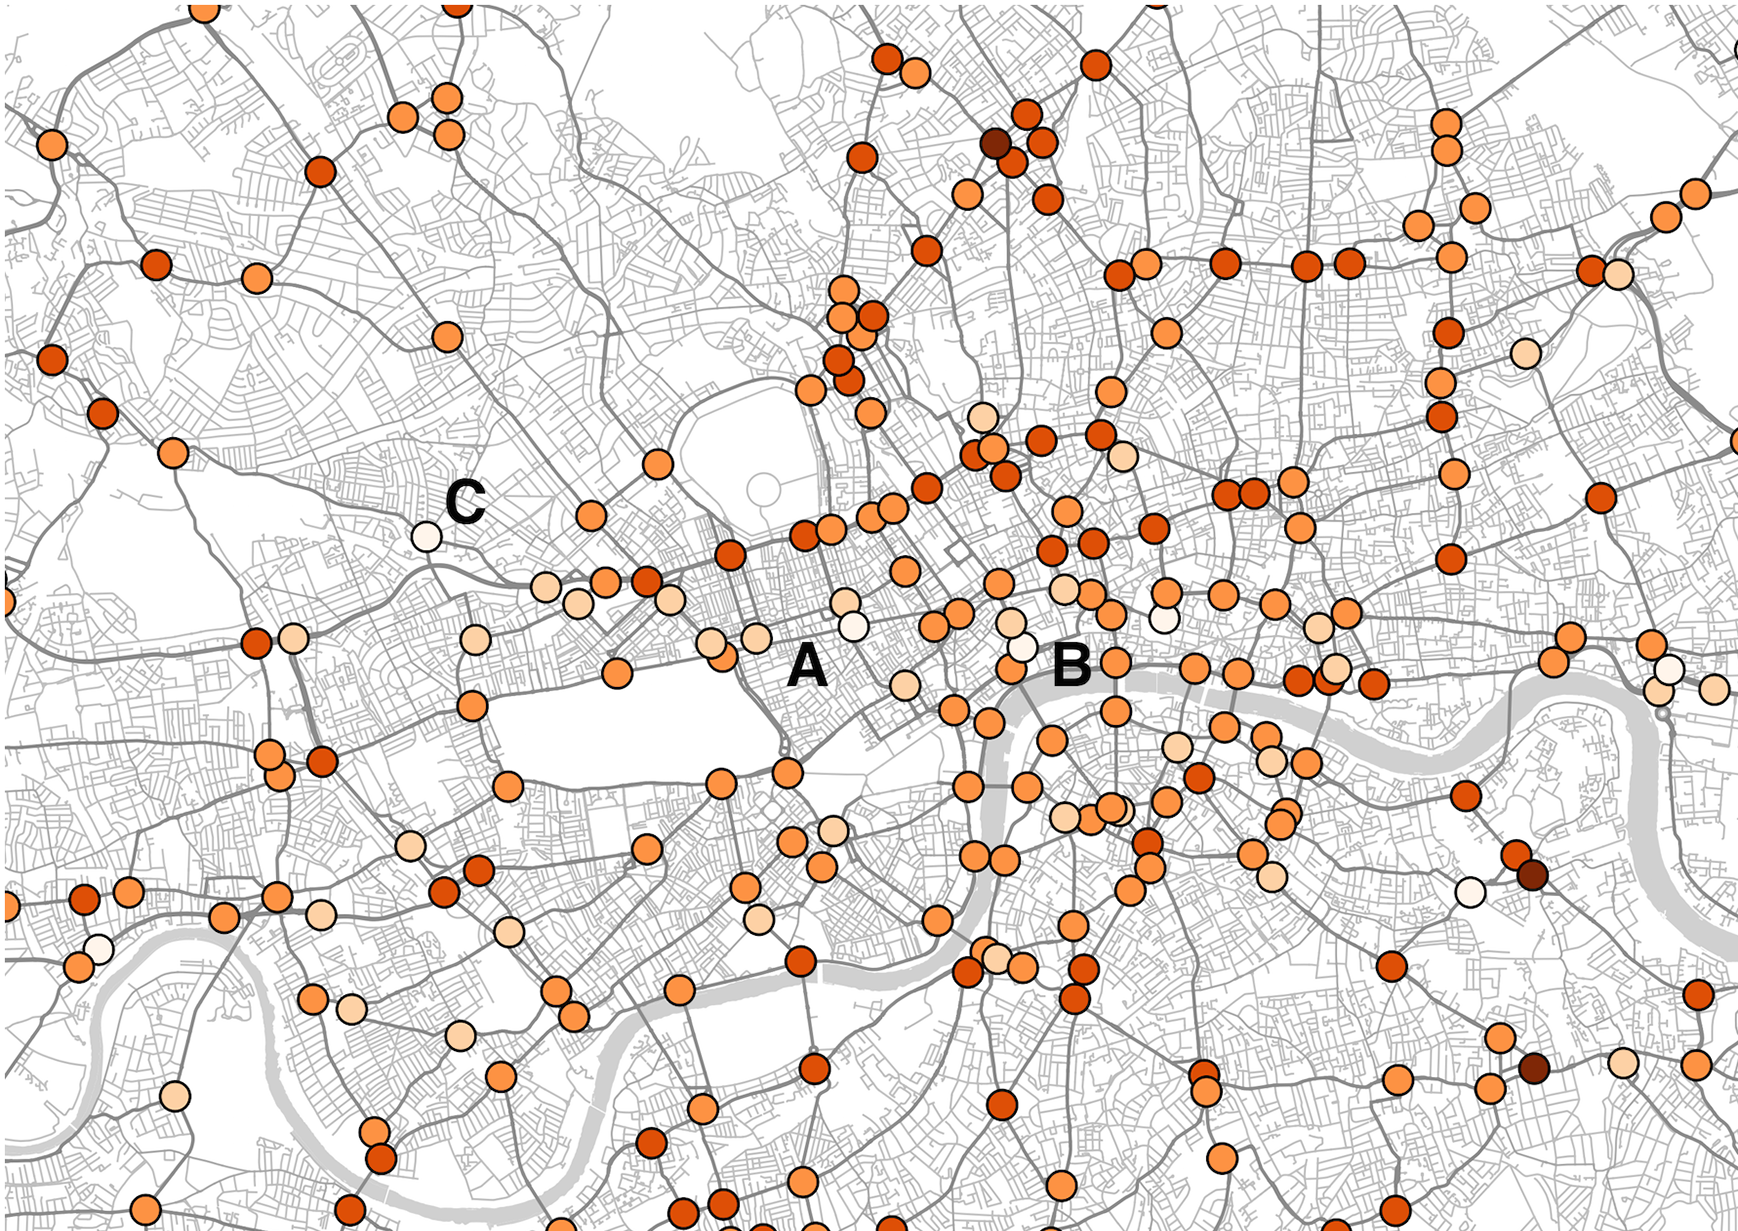
\includegraphics[width=4cm, height=2.5cm]{img/traffic.png}\\
            Traffic
            \column{.5\textwidth}
            \centering
            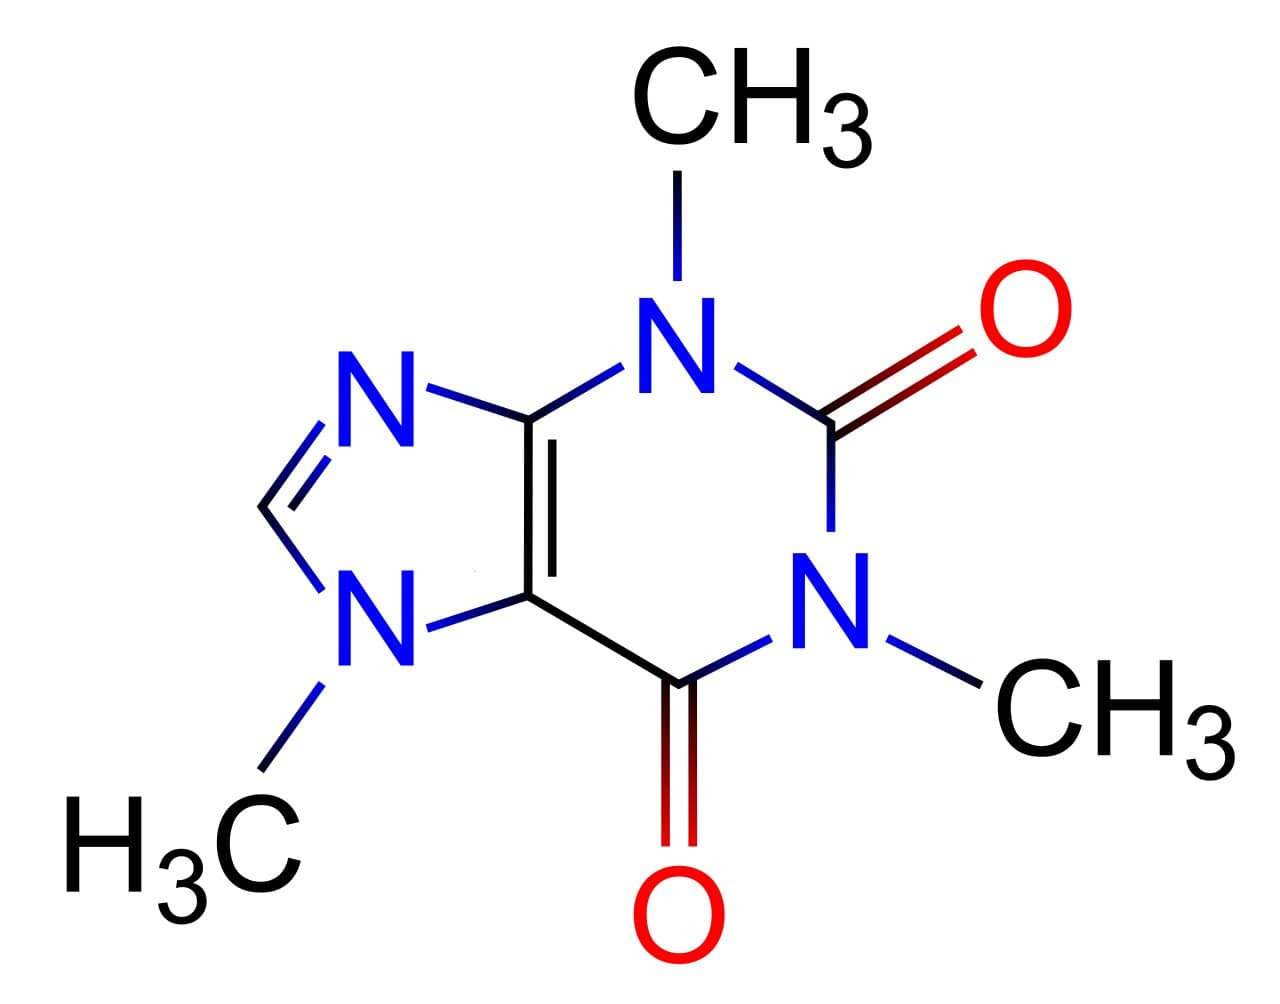
\includegraphics[width=3cm, height=2cm]{img/Caffeine.jpg}\\
            Chemistry
        \end{columns}
    \centering
    \vskip.5cm
    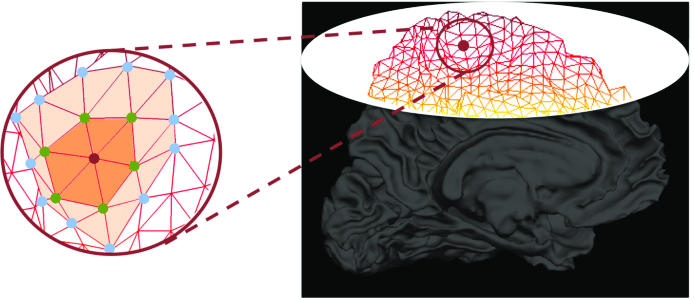
\includegraphics[width=5.5cm, height=2.5cm]{img/coritcal_mesh.png}\\
    Neuroscience
\end{frame}

\begin{frame}[t]
    \frametitle{Problem Setup}
    \begin{columns} % align columns
        \begin{column}{.48\textwidth}
            \begin{minipage}[c][.9\textheight][c]{.98\textwidth}
                \begin{center}    
                    \vskip0.25cm
                    Grid Data
                    \vskip0.05cm
                    \begin{figure}
                        \begin{overprint}
                        \onslide<1>\centering 
\includegraphics[width=5.4cm, height=6cm]{img/van_gogh.jpg}
                        \onslide<2>\centering 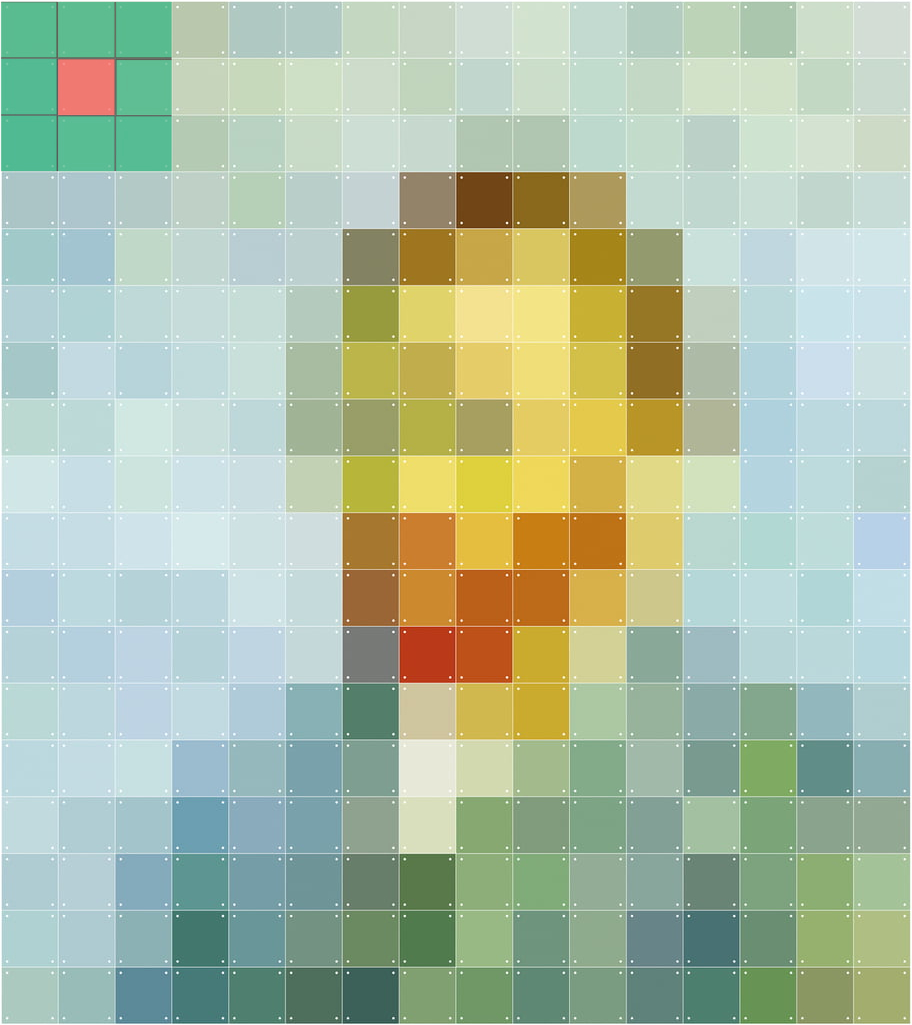
\includegraphics[width=5.4cm, height=6cm]{img/van_gogh_1.jpg}
                        \onslide<3->\centering 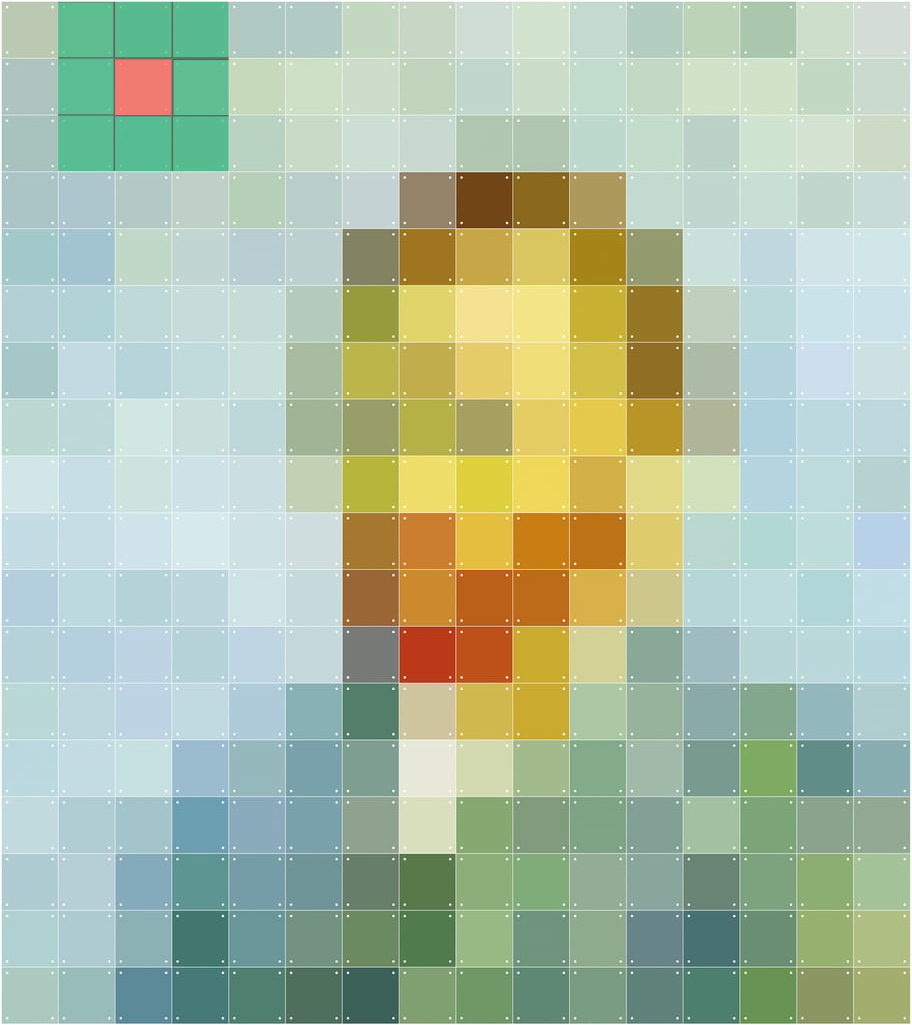
\includegraphics[width=5.4cm, height=6cm]{img/van_gogh_2.jpg}
                        \end{overprint}
                    \end{figure}
                \end{center}
            \end{minipage}
        \end{column}%
        \begin{column}{.48\textwidth}
            \begin{minipage}[c][.9\textheight][c]{.98\textwidth}
                \begin{center}    
                    \vskip-0.225cm
                    Graph Data
                    \vskip0.5cm
                    \begin{figure}
                        \begin{overprint}
                        \onslide<4>\centering 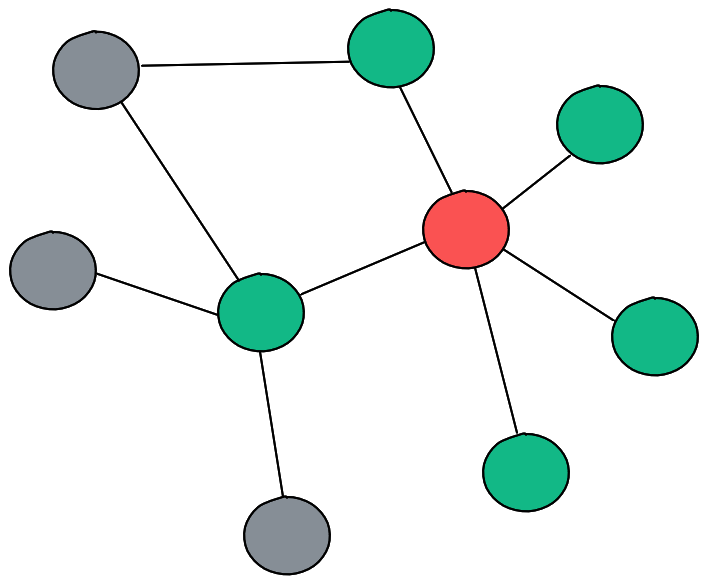
\includegraphics[width=6cm, height=5cm]{img/graph_conv_1.png}
                        \onslide<5>\centering 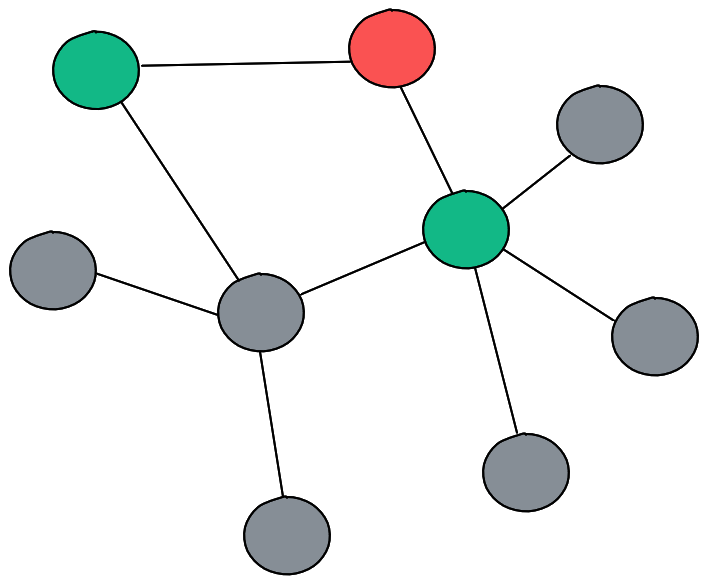
\includegraphics[width=6cm, height=5cm]{img/graph_conv_2.png}
                        \end{overprint}
                    \end{figure}
                \end{center}
            \end{minipage}
        \end{column}%
    \end{columns}
\end{frame}


\subsection{Graph Neural Networks}

\begin{frame}[t]
    \frametitle{Graph Neural Networks}
    \begin{center}
        \begin{figure}
            \begin{overprint}
                \onslide<1>\centering 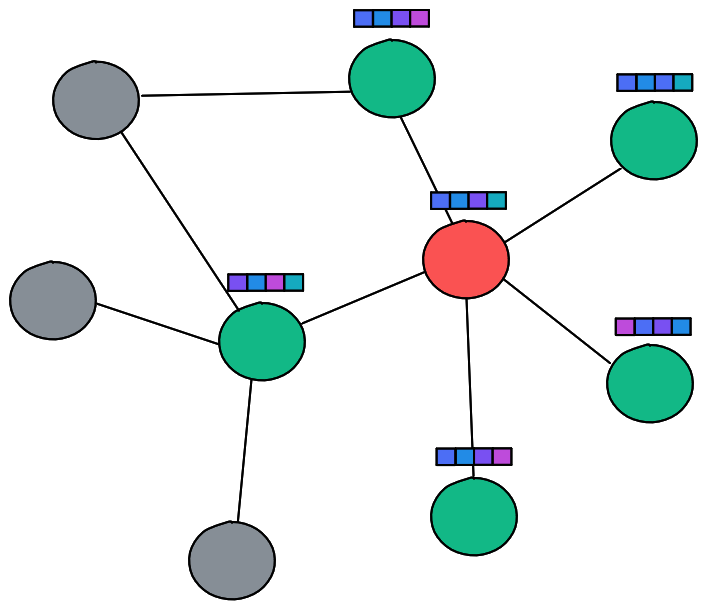
\includegraphics[width=7cm, height=6cm]{img/gnn_1.png}
                \onslide<2>\centering 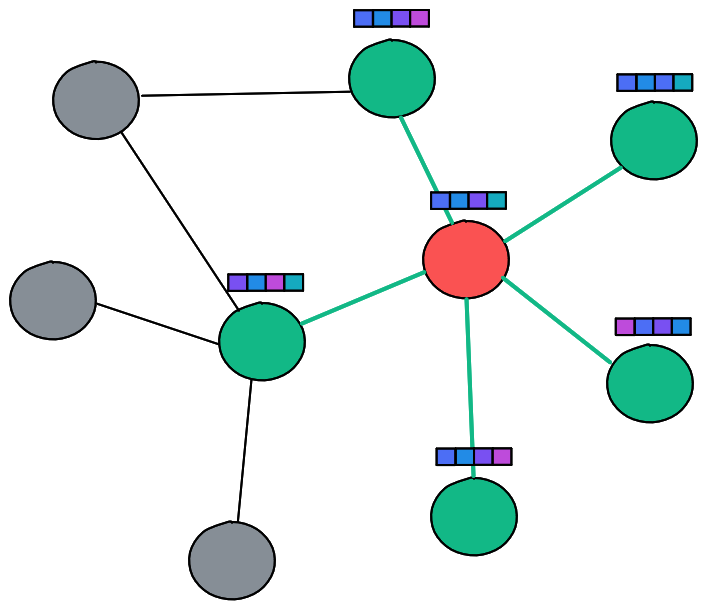
\includegraphics[width=7cm, height=6cm]{img/gnn_2.png}
                \onslide<3->\centering 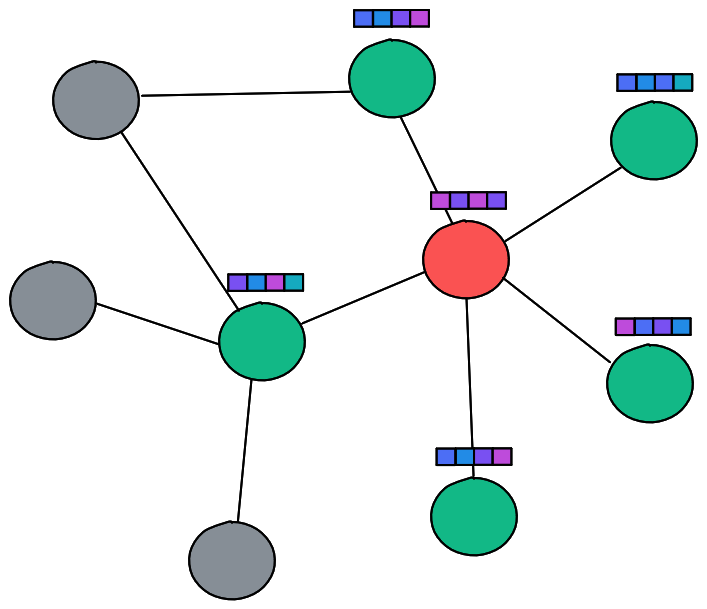
\includegraphics[width=7cm, height=6cm]{img/gnn_3.png}
            \end{overprint}
        \end{figure}
    \end{center}
\end{frame}

%------------------------------------------------
\section{GATs}
%------------------------------------------------
\subsection{GAT Architecture}
\subsection{Visual Explanation}
\subsection{Attention Mechanisms}

\begin{frame}[t]
    \frametitle{GAT Layer}
    \begin{tabular}{p{5.5cm} p{7cm}}
        \vspace{0pt}
        $h_i \in \mathbb{R}^F$, $h_i' \in \mathbb{R}^{F'}$ \\
        \uncover<1->{
            feature weight matrix $\mathbf{W} \in \mathbb{R}^{F' \times F}$ \\
            \textbf{shared} attention mechanism \\
            $a: \mathbb{R}^{F'} \times \mathbb{R}^{F'} \rightarrow \mathbb{R}$\\
            }
        \uncover<2->{
        attention coefficients\\
        $e_{ij} = a(\mathbf{W}h_i, \mathbf{W}h_j)$\\}
        \uncover<3->{
        normalized attention coefficients\\
        $\alpha_{ij} = \textup{softmax}_j(e_{ij})$
        \\}
        \uncover<5->{
        output with nonlinearity $\sigma$\\
        $h_i' = \sigma(\mathlarger{\sum}_{j\in \mathcal{N}_i} \alpha_{ij}\mathbf{W}h_j)$}
        & 
        \begin{overprint}
            \vspace{-6cm}
            \onslide<1> 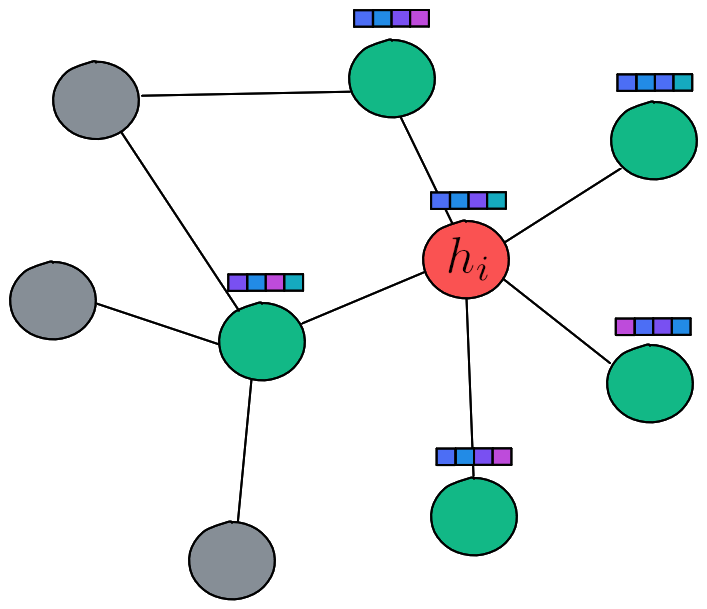
\includegraphics[width=7cm, height=6cm, valign=t]{img/gnn_1_hi.png}
            \onslide<2>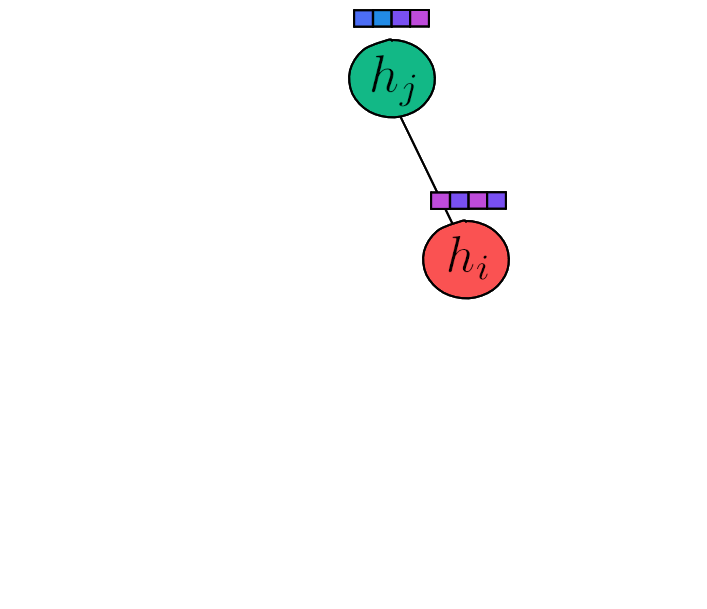
\includegraphics[width=7cm, height=6cm, valign=t]{img/gat_neighbors.png}
            \onslide<3>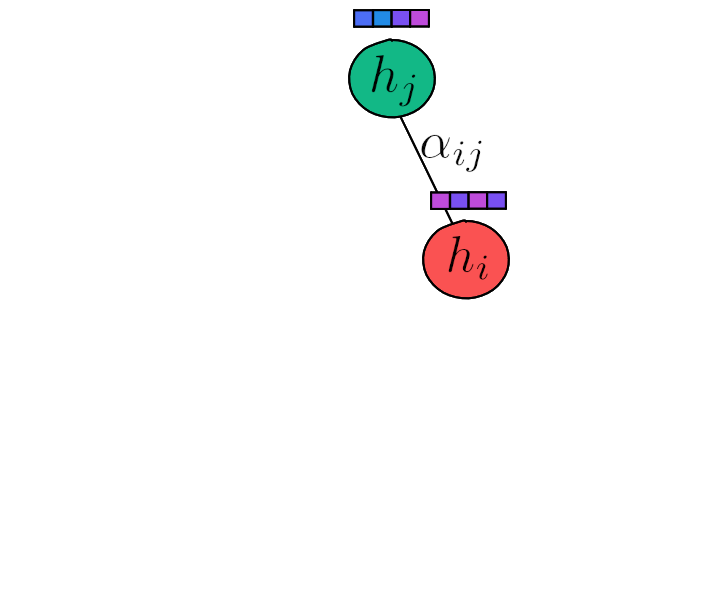
\includegraphics[width=7cm, height=6cm, valign=t]{img/gat_neighbors_weighted.png}
            \onslide<4>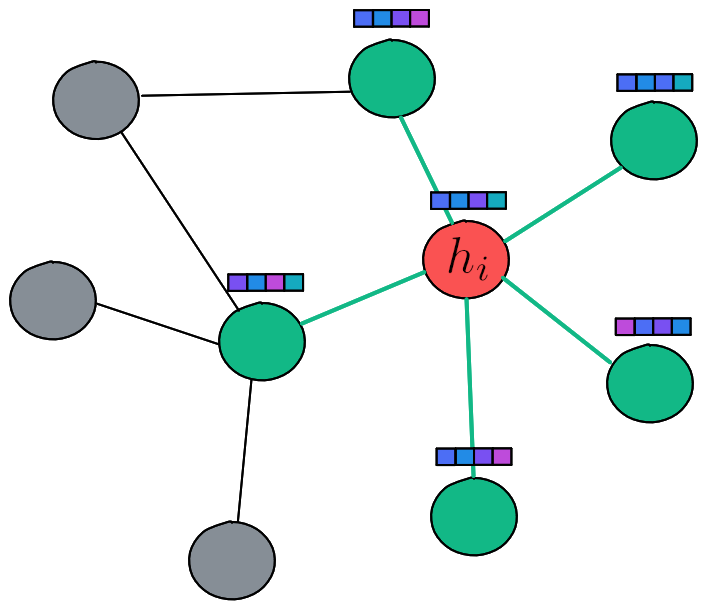
\includegraphics[width=7cm, height=6cm]{img/gnn_2_hi.png}
            \onslide<5>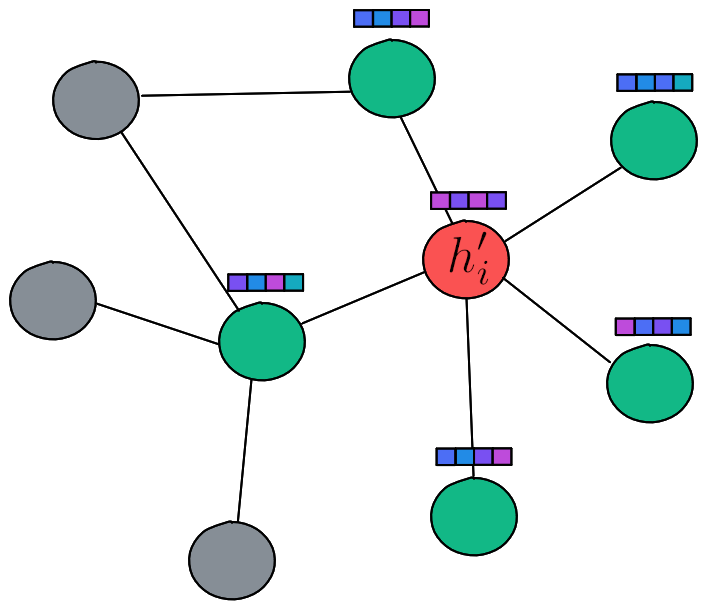
\includegraphics[width=7cm, height=6cm]{img/gnn_3_hi_prime.png}
        \end{overprint}
    \end{tabular}
\end{frame}

\begin{frame}
    \frametitle{Multi-Head Attention}
    \begin{figure}
        \centering
        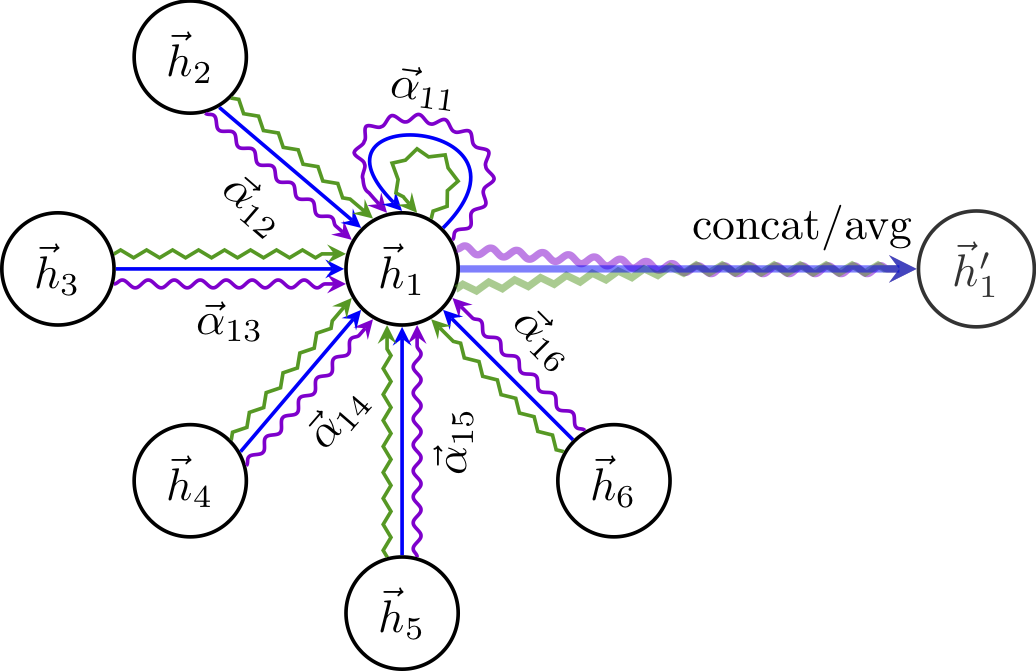
\includegraphics[width=9.5cm, height=6cm, valign=t]{img/multi_head.png}
        \subcaption*{\color{gray}{Veličković \emph{et al.} 2018}}
    \end{figure}
\end{frame}

%------------------------------------------------
\section{Applications}
%------------------------------------------------
\subsection{Improvements over previous methods}
\begin{frame}
    \frametitle{Improvements over previous methods}
    \begin{itemize}
        \item applicable for various graphs (directed, undirected, different node degrees)
        \vspace{1em}
        \item shared attention mechanism allows usage for \textbf{inductive} learning tasks
        \vspace{1em}
        \item previous inductive methods did not include all neighbors
        \vspace{1em}
        \item attention weights lead to more interpretability
    \end{itemize}
\end{frame}

\subsection{Results using GATs}
\begin{frame}
    \frametitle{Results using GATs}
    \begin{itemize}
        \item Classification of Brain Surface Areas (\href{https://openreview.net/forum?id=rkKvBAiiz}{Cucurull \emph{et al.}, 2018})
        \vspace{1em}
        \item Explainable Text Models 
            \href{https://www.semanticscholar.org/paper/A-First-Look\%3A-Towards-Explainable-TextVQA-Models-Rao-Zhen/6b81ee53fe89692cd0900182333a9e0212caa9ca}{(Rao \emph{et al.}, 2021)}
    \end{itemize}
\end{frame}

\begin{frame}
    \frametitle{Brain Mesh Segmentation}
    \begin{figure}
        \centering 
        \begin{overpic}[trim={0 0 0 5}, width=12cm, height=6.77cm]{img/brain_mesh.PNG}
            \put (35, -1) {\color{gray}{Cucurull \emph{et al.} 2018}}
           \end{overpic}
    \end{figure}
\end{frame}

\begin{frame}
    \frametitle{Explainable Text Visual Question Answering Models}
    \begin{figure}
        \centering 
        \begin{overpic}[trim={0 0 0 0}, width=6.7cm, height=6.77cm]{img/text_1.PNG}
            \put (27.5, -2.5) {\color{gray}{Rao \emph{et al.} 2021}}
           \end{overpic}
    \end{figure}
\end{frame}

\begin{frame}
    \frametitle{Explainable Text Visual Question Answering Models}
    \begin{figure}
        \centering 
        \begin{overpic}[trim={0 0 0 0}, width=11.2cm, height=6.77cm]{img/text_2.PNG}
            \put (37, -1.95) {\color{gray}{Rao \emph{et al.} 2021}}
           \end{overpic}
    \end{figure}
\end{frame}

\begin{frame}
    \frametitle{Explainable Text Visual Question Answering Models}
    \begin{figure}
        \centering 
        \begin{overpic}[trim={0 0 0 0}, width=9.2cm, height=6.77cm]{img/text_3.PNG}
            \put (34.2, -2.43) {\color{gray}{Rao \emph{et al.} 2021}}
           \end{overpic}
    \end{figure}
\end{frame}

%------------------------------------------------
\section{Discussion}
%------------------------------------------------
\subsection{Limitations}
\subsection{(Related Work)}
\begin{frame}
    \frametitle{Related Work and Limitations}
    \begin{itemize}
        \item Benchmarking Graph Neural Networks \href{https://arxiv.org/abs/2003.00982}{(Dwivedi \emph{et al.} 2020)}
        \vspace{1em}
        \item Do we need deep graph neural networks? \href{https://towardsdatascience.com/do-we-need-deep-graph-neural-networks-be62d3ec5c59}{(Bronstein 2020)}
    \end{itemize}
\end{frame}

\begin{frame}
    \frametitle{Benchmarking GNNs}
    \begin{center}
         \Large Cora and Citeseer are not large enough
    \end{center}    
\end{frame}

\begin{frame}
    \frametitle{Benchmarking GNNs}
    \begin{figure}
        \centering 
        \begin{overpic}[trim={10 0 0 20}, width=13cm, height=6.77cm]{img/benchmark_dwivedi.PNG}
            \put (37, 13) {\color{gray}{Dwivedi \emph{et al.} 2020}}
        \end{overpic}
    \end{figure}
\end{frame}

\begin{frame}
    \frametitle{Benchmarking GNNs}
    \begin{center}
         \Large different taks favor different models
    \end{center}    
\end{frame}

\begin{frame}
    \frametitle{Benchmarking GNNs}
    \begin{figure}
        \centering 
        \begin{overpic}[trim={5 0 0 20}, width=13cm, height=7cm, valign=t]{img/benchmark_gat_worse.PNG}
            \put (37, 11) {\color{gray}{Dwivedi \emph{et al.} 2020}}
        \end{overpic}
    \end{figure}
\end{frame}

\begin{frame}
    \frametitle{Going deep with GNNs}
    \begin{center}
         \Large How far can we go with GATs?
    \end{center}    
\end{frame}

\begin{frame}
    \frametitle{Going deep with GNNs}
    \begin{figure}
        \centering 
        \begin{overpic}[width=10cm, height=6.77cm]{img/oversmoothing.png}
        \end{overpic}
    \end{figure}
\end{frame}

\begin{frame}
    \frametitle{Going deep with GNNs}
    \begin{figure}
        \centering 
        \begin{overpic}[trim={10 0 0 20}, width=11cm, height=6.77cm]{img/bottleneck.png}
            \put (37, 1) {\color{gray}{Alon \& Yahav 2021}}
           \end{overpic}
    \end{figure}
\end{frame}
%------------------------------------------------
\section{References}
%------------------------------------------------

\begin{frame}
    \frametitle{References}
    \footnotesize{
        \begin{thebibliography}{99}

        \bibitem {}{Veli{\v{c}}kovi{\'{c}} \emph{et al.} 2018}
        \newblock Graph Attention Networks
        \newblock {\href{https://arxiv.org/abs/1710.10903}{\emph{arXiv} 1710.10903}}
        \newblock {}{\href{https://github.com/PetarV-/GAT}{github.com/PetarV-/GAT}}\\
        %--------------------------------------------
        \bibitem {}{Cucurull \emph{et al.} 2018}
        \newblock Convolutional neural networks for mesh-based parcellation of the cerebral cortex
        \newblock {}{\href{https://2018.midl.io/scientific-program.html}{MIDL 2018 Conference Submission}}\\
        \href{https://openreview.net/forum?id=rkKvBAiiz}{https://openreview.net/forum?id=rkKvBAiiz}\\
        %--------------------------------------------
        \bibitem {}{Rao \emph{et al.} 2021}
        \newblock A First Look: Towards Explainable TextVQA Models via Visual and Textual
        Explanations
        \newblock {\href{https://arxiv.org/abs/2105.02626}{\emph{arXiv} 2105.02626}}
        \end{thebibliography}
    }
\end{frame}

\begin{frame}
    \frametitle{References}
    \footnotesize{
        \begin{thebibliography}{99}

        \bibitem {}{Dwivedi \emph{et al.} 2020}
        \newblock Benchmarking Graph Neural Networks
        \newblock {\href{https://arxiv.org/abs/2003.00982}{\emph{arXiv} 2003.00982}}\\        %--------------------------------------------
        \bibitem {}{Bronstein 2020}
        \newblock Do we need deep graph neural networks?
        \newblock {}{\href{https://towardsdatascience.com/do-we-need-deep-graph-neural-networks-be62d3ec5c59}{https://towardsdatascience.com/do-we-need-deep-graph-neural-networks-be62d3ec5c59}}\\
        %--------------------------------------------
        \bibitem {}{Alon \& Yahav 2021}
        \newblock On the Bottleneck of Graph Neural Networks and its Practical Implications
        \newblock {\href{https://arxiv.org/abs/2006.05205}{\emph{arXiv} 2006.05205}}
        \end{thebibliography}
    }
\end{frame}


\end{document} 